\section{Background}
\label{sec:background}

In this section, we present background on edge computing, its computing models and failure models.
We also present EdgeCloudSim, the simulator used in our later simulation.

\subsection{Edge Computing}
Cloud computing and mobile computing are now used everywhere.
After several decades of sustained effort by many researchers, both of them have
solid core concepts, techniques and mechanisms. Many applications running on mobile devices nowadays
leverage cloud computing to overcome the resource limits of mobile devices. However,
long WAN delays in the critical path of user interaction can hurt the application
performance and responsiveness~\cite{cloudlets09}.

{
\begin{figure}[th]
\begin{center}
	\centerline{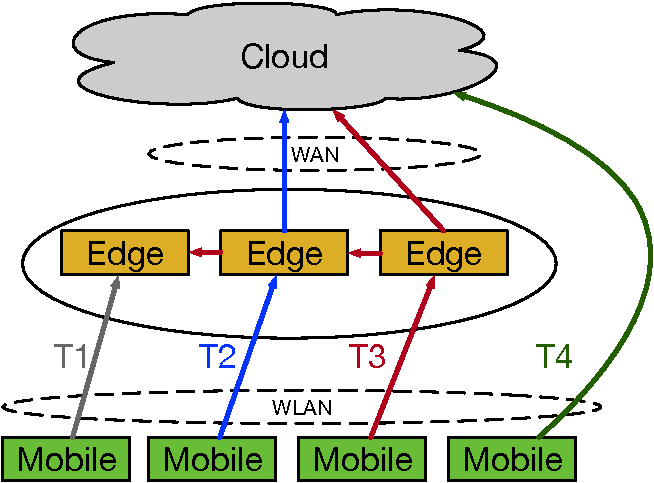
\includegraphics[width=2.5in]{Figures/computing-models.pdf}}
	\mycaption{fig-computing-models}{Computing Models}
	{
		Four different computing models under different usages of edge devices.
		Type 1 means mobile device uses one edge device only. Edge device
		can also push computation to cloud in type 2. In type 3, edge devices
		can do load-balancing. Type 4 is the original two-tier architecture,
		mobile contact with cloud only.
	}
\end{center}
\end{figure}
}

{
\begin{figure}[th]
\begin{center}
	\centerline{\includegraphics[width=2.5in]{Figures/edgecloudsim.pdf}}
	\mycaption{fig-edgecloudsim}{EdgeCloudSim Layered Architecture}
	{
		CloudSim provides the fundamental simulation support.
		Above that, EdgeCloudSim adds mobility simulation module
		and network simulation module.
	}
\end{center}
\end{figure}
}



Edge computing is a new computing paradigm which moves the computation closer to the mobile devices.
The reousrce in the proximity used in edge computing can be a network resource or a computational resource
in between mobile devices and the cloud. Satyanarayanan et al.~\cite{cloudlets09} introduced the concept
of cloudlet, which is a trusted, resource-rich computer or cluster of computers that's well-connected to
the Internet and available for use by nearby mobile devices. Cloudlet has been extensively discussed in the
literatures~\cite{edge-computing, Cloudlets12,hu-apsys16,ChaufournierSLN17}.

An edge computing infrastructure can be composed of many edge servers and management system softwares.
The management system needs to decide where to offload a task, and how to ensure reliability and availability
in case of failures. Recent work \cite{hu-apsys16,COMET} show that application partition schema, and network latency
both have significant impacts on edge computing performance.

\subsection{Computing Models}
\label{sec:computing-models}
Edge computing offers more possibilities for current mobile-cloud computing architecture.
Figure~\ref{fig-computing-models} presents four computing models. Type 4 is the original
two-tier architecture, where mobile devices communicate with cloud only. With the introduction of
edge devices, it makes type 1 to type 3 possible. In type 1, mobile device contacts with only one edge device.
This is benefical for mobile devices with low mobility. Compared with type 1, edge devices in type 2 can
push computation to cloud, whenever edge devices think offloading can improve performance. Type 3 offers
more flexibility by load-balancing jobs among multiple edge devices.

\subsection{Failure Models}
\label{sec:failure-models}
While benefical from the performance aspect, edge computing also introduces more
{\em failure domains} into current computing framework. Since we are interested
in how edge devices can impact the whole performance, we will mainly focus on
the {\em additional} failure domains brought by edge computing. Namely:
\begin{enumerate}
\item Edge device crash
\item Network failure between mobile device and edge device
\item Network failure among multiple edge devices
\item Network failure between edge device and cloud
\end{enumerate}

During runtime, we assume the senders of the communication channel are able to detect failures
of receivers by software timeout. Edge devices and cloud will also use heartbeat
messages to detect liveness. Despite all these failures, the goal of resilient
edge computing is to provide high availability and reliability guarantees to
applications running on mobile devices.

\subsection{EdgeCloudSim}
Developing a set of system software for edge computing is not an easy process due
to the complexity of various application requirments and different mobile devices.
Therefore it is better to have a basic understanding of what edge computing can provide
before doing real system implementation.

EdgeCloudSim~\cite{edgecloudsim} is a recent simulator designed for edge computing.
EdgeCloudSim is based on CloudSim~\cite{cloudsim}, which is a mature cloud computing simulation framework.
CloudSim is mainly designed for evaluating the performance of the data centers, thus lack the essential
properties to model edge devices and mobile devices. To be able to simulate edge computing, EdgeCloudSim
extends CloudSim by adding the following features: (i) a queueing model to represent the delay in WLAM and WAN,
(ii) a mobility model, and (iii) a new CPU utilization model for VMs~\cite{edgecloudsim}.
Figure~\ref{fig-edgecloudsim} shows its layered architecture.

EdgeCloudSim provides three different architectures: single-tier, two-tier and two-tier with load-balancing.
They map to type 1, type 2 and type 3 as illustrated in Figure~\ref{fig-computing-models} respectively.
EdgeCloudSim is also able to limit network bandwidth, simulate mobility of mobile devices.
We present detailed evaluation using EdgeCloudSim with different computing models in section~\ref{sec:simulation}.
